\documentclass{standalone}
\usepackage{tikz}
\usetikzlibrary{calc}
\usetikzlibrary{arrows.meta, positioning, decorations.pathmorphing,decorations.pathreplacing, shapes.misc, fadings, shadows}
\usepackage{pgf}
\usepgflibrary{fpu}
\begin{document}


    % \begin{tikzpicture}[node distance=1.5cm, scale=0.7, every node/.style={scale=0.7}]

    % % Define color gradient
    % \begin{scope}
    % \pgfdeclarehorizontalshading{arrowgradient}{1cm}{rgb(0cm)=(0.8,0.8,1); rgb(1cm)=(1,1,1)}
    % \end{scope}
    
    % % Nodes
    % \node[draw,rectangle,fill=red!70, minimum width=5cm,align=center, minimum height=4cm] (system) {\huge Athlète \\~\\ (Musculaire,\\Cardiovasculaire,\\neuromusculaire...)};
    % \node[draw,rectangle, above left =-0.5cm and 1.5cm of system,align = center,minimum size=2.6cm] (env) {Environnement\\(externe)};
    % \node[draw,rectangle, left= 1.5cm of system, minimum size=2.6cm] (energie) {Energie stockée};
    % \node[draw,fill=blue!50,rectangle, below left= -0.5cm and 1.5cm of system, minimum size=2.6cm] (o2) {Oxygène};
    % \node[draw,fill=yellow!50,rectangle, above =  of system, minimum size=1.5cm] (neuro) {Activation neuromusculaire};
    % \node[draw,fill=green,align=center,rectangle, right= 3cm of system, minimum size=1.5cm] (output) {Charge Externe mesurée : \\Puissance,\\Vitesse,\\Distance,\\ ...};
    % \node[draw,circle,fill=orange, below left=2cm and -.5cm of system, minimum size=1.5cm] (hr) {HR};
    % \node[draw,circle,fill=orange, below right=2cm and -0.5cm of system, minimum size=1.5cm] (rpe) {RPE};
    % \node[draw,circle,fill=orange, below =2cm of system, minimum size=1.5cm] (lt) {Lactate};
    % \node[below of= lt] (measure) {Mesures de l'état du système \\ ~ Charge interne };
    % \node[draw,circle,above right= of system,align = center, sloped,text =black,text width = 2cm] (eff) {Énergie produite par le muscle};

    
    % % Arrows
    % \draw[->] (env) -- (system);
    % \draw[->] (energie) -- (system);
    
    % % Special arrow with gradient
    % % \draw[->, draw=none] (o2) -- (system) node[midway, above, draw=none] {VO2Max};
    % % \draw[decorate,decoration={snake,segment length=15pt, amplitude=1mm, pre length=1mm,post length=1mm}] (o2) -- (system);
    % % \shade[shading=arrowgradient, shading angle=0] ($(o2) + (-1cm,0.25cm)$) -- ($(o2) + (-1cm,-0.25cm)$) -- ($(system) + (-2cm,-0.15cm)$) -- ($(system) + (-2cm,0.15cm)$) -- cycle;
    
    % \begin{scope}
    %     \shade[left color=blue, right color=blue!20, opacity=0.5]
    %     (o2.east |- o2.north) -- 
    %     (o2.east |- o2.south) -- 
    %     (system.west |- system.center) -- 
    %     cycle;
    %     \node[opacity=1, above right=0.4cm and 0.5cm of o2.east, rotate=66, text=black] {\scriptsize VO2Max};
    % \end{scope}

    % \begin{scope}
    %     \shade[left color=red, right color=green!50, opacity=0.7]
    %     (system.east |- system.north) -- 
    %     (system.east |- system.south) -- 
    %     (output.west |- output.center) -- 
    %     cycle;
    %     \node[opacity=1,right = 2.5 cm of system.center,align = center, sloped,text =black,text width = 2cm] {\scriptsize Efficacité de la transmition};
    %     % \node[opacity=1,below right = -.5cm and 1.5 cm of system.south,align = center, rotate = 90, sloped,text = black,text width = 2.5cm] {\scriptsize Énergie produite\\par le muscle};
    % \end{scope}
    % % \draw[fill=blue, draw=none, opacity=0.2] 
    % %     (o2.east |- o2.north) -- 
    % %     (o2.east |- o2.south) -- 
    % %     (system.west |- system.center) -- 
    % %     cycle node[opacity=1,right= 0.05cm of o2.east,rotate = 40] {VO2Max};

    % % \draw[->] (system) -- (output) node[midway,align=center, above = 1cm, sloped, text width=4cm] {Efficacité de la transmition} 
    % %\\(dépend du frottement,\\technique de courses,\\pédalage, aérodynamisme, vélo)} 
    % %rotation of 90                            
    
    % \draw[->] (hr) -- (system);
    % \draw[->] (rpe) -- (system);
    % \draw[->] (lt) -- (system);
    % \draw[->] (neuro) -- (system);
    % \draw[->] (eff) -- (system.north east);
    
    % % Grouping measures
    % \draw[dotted,color = red] ($(hr.north west)+(-0.4,0.4)$) rectangle ($(rpe.south east)+(0.6,-0.6)$);
    % \node[draw,color = red,dotted,left=0.1cm of measure] {  };
    
    % \end{tikzpicture}
    
    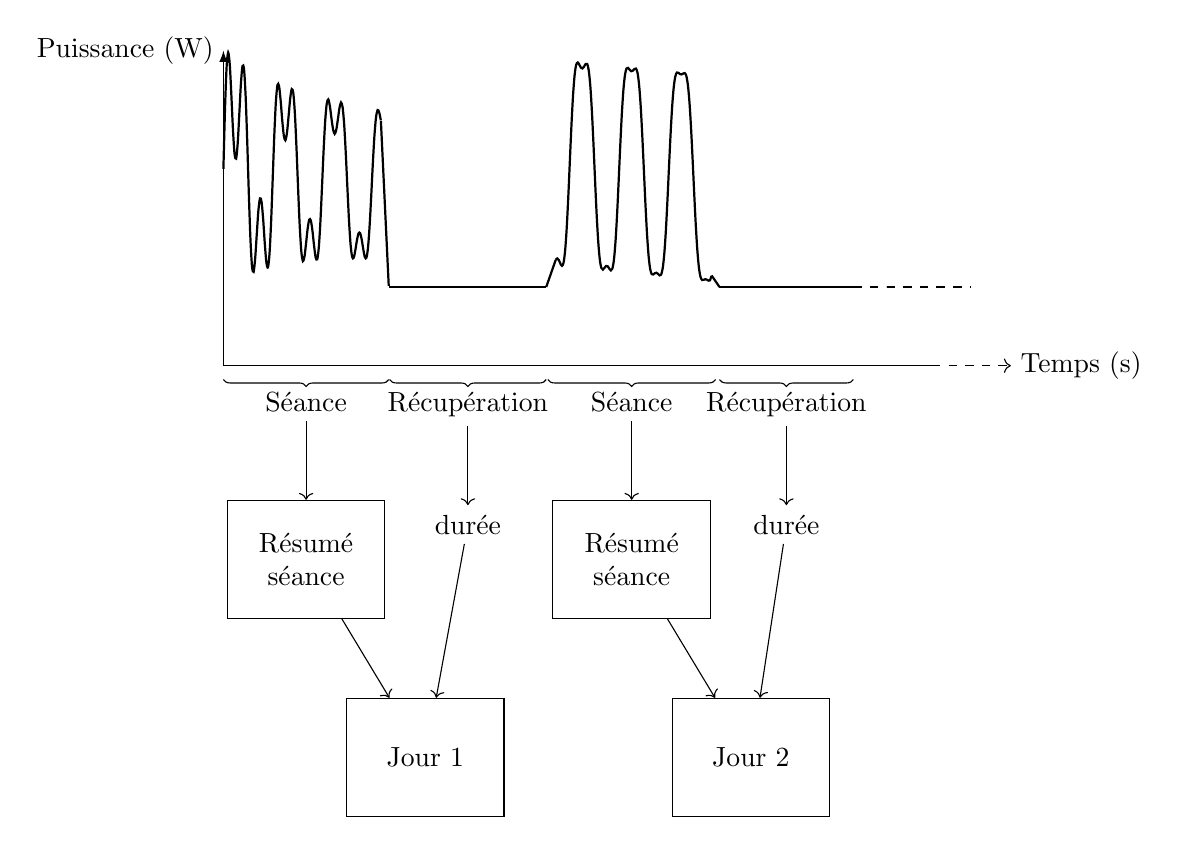
\begin{tikzpicture}
        \tikzset{
            axis/.style={->, >=latex},
            graph/.style={thick, smooth},
            box/.style={draw, rectangle, minimum width=2cm, minimum height=1.5cm, align=center},
        }
        
        
        \begin{scope}[yshift=6cm,xshift=3cm]
            \draw[axis] (0,-1) -- (0,3) node[left] {Puissance (W)};
            \draw (0,-1) -- (9,-1);
            \draw[dashed,->] (9,-1) -- (10,-1) node[right] {Temps (s)};
            
            % Enable FPU for calculations
            \draw[graph] plot[variable=\x,domain=0:2,samples=100] 
                (\x,{1.5-0.1*\x+1*sin(30*\x r)/(1+\x) + sin(10*\x r)});
           
            % make a smooth transition to 0
            % Transition region
            \draw[graph] plot[variable=\x,domain=2:2.1,samples=100] 
            (\x,{ (1.5-0.1*2+1*sin(30*2 r)/(1+2) + sin(10*2 r)) * (2.1-\x)/0.1 
            + (0+0.01*sin(40*2.1 r)) * (\x-2)/0.1 });

            \draw[graph] plot[variable=\x,domain=2.1:4.1,samples=100] 
                (\x,{0.00*sin(40*\x r)});
            
            % Transition region
                \draw[graph] plot[variable=\x,domain=4.1:4.22,samples=100] 
                (\x,{ (0.00*sin(40*4.1 r)) * (4.22-\x)/0.12 
                + (2-0.1*4.22+1.5*sin(30*4.22 r)/(1+4.22) + 1.5*sin(10*4.22 r)) * (\x-4.1)/0.12 });
            

            
            \draw[graph] plot[variable=\x,domain=4.22:6.2,samples=100] 
            (\x,{2-0.1*\x+1.5*sin(30*\x r)/(1+\x) + 1.5*sin(10*\x r)});

            % Transition region
            \draw[graph] plot[variable=\x,domain=6.2:6.3,samples=100] 
            (\x,{ (2-0.1*6.2+1.5*sin(30*6.2 r)/(1+6.2) + 1.5*sin(10*6.2 r)) * (6.3 - \x)/0.1
            + 0 * (\x-6.2)/0.1 });
            % + (0.05*sin(30*6.3 r)) * (\x-6.2)/0.1 });

            \draw[graph] plot[variable=\x,domain=6.3:8,samples=100] 
                % (\x,{0.01*sin(30*\x r)});
                (\x,{0});

            \draw[graph,dashed] plot[variable=\x,domain=8:9.5,samples=100] 
                (\x,{0});

                \draw[decoration={brace,mirror,raise=5pt},decorate] (0,-1) -- node[below=6pt] (s1) {Séance} (2.1,-1);
                \draw[decoration={brace,mirror,raise=5pt},decorate] (2.11,-1) -- node[below=6pt] (r1) {Récupération} (4.1,-1);
                \draw[decoration={brace,mirror,raise=5pt},decorate] (4.12,-1) -- node[below=6pt] (s2) {Séance} (6.25,-1);
                \draw[decoration={brace,mirror,raise=5pt},decorate] (6.3,-1) -- node[below=6pt] (r2) {Récupération} (8,-1);

                \node[below =1cm of s1,box] (res1) {Résumé\\séance};
                \node[below= 1cm of s2,box] (res2) {Résumé\\séance};
                \node[below =1cm of r1] (rer1) {durée};
                \node[below =1cm of r2] (rer2) {durée};

                \draw[->] (r1) -- (rer1);
                \draw[->] (r2) -- (rer2);
            
                \draw[->] (s1) -- (res1);
                \draw[->] (s2) -- (res2);

                \node[box,below right = 1cm and -0.5cm of res1] (j1) {Jour 1};
                \node[box,below right = 1cm and -0.5cm of res2] (j2) {Jour 2};

                % Arrows
                \draw[->] (res1) -- (j1);
                \draw[->] (res2) -- (j2);
                \draw[->] (rer1) -- (j1);
                \draw[->] (rer2) -- (j2);




            % \node[anchor=north east] at (10,3) {RPE: G};
            % \node[anchor=south west, text width=3cm, align=left] at (0,3) {Perception / Monse de l'athlète};
        \end{scope}
    \end{tikzpicture}


\end{document}
